\documentclass[authoryear,preprint,review,10pt]{elsarticle}
\usepackage{amssymb,amsthm,amsmath,setspace}
\usepackage{url,color}
\usepackage{lineno}
\usepackage[labelfont=bf,format=hang,textfont=it]{caption}
\usepackage{graphicx}
\usepackage{microtype}
\usepackage[letterpaper,text={15cm,23cm}]{geometry}
\usepackage{natbib}
\usepackage{hyperref}

%% for internal use
\newcommand{\fixme}[1]{\emph{\marginpar{FIXME} (#1)}}
\newcommand{\readme}[1]{\emph{\marginpar{README} (#1)}}

\definecolor{Red}{rgb}{0.5,0,0}
\definecolor{Blue}{rgb}{0,0,0.5}
\hypersetup{%
  pdftitle = {Real-time change detection},
  pdfsubject = {},
  pdfkeywords = {monitoring, time series, MODIS, NDVI},
  pdfauthor = {Jan Verbesselt, Achim Zeileis},
  %% change colorlinks to false for pretty printing
  colorlinks = {true},
  linkcolor = {Blue},
  citecolor = {Blue},
  urlcolor = {Red},
  hyperindex = {true},
  linktocpage = {true},
}


\journal{Remote Sensing of Environment}

\begin{document}
%% \linenumbers
\begin{frontmatter}

    \title
    {
    Real-time land cover disturbance detection \\ using satellite image time series
    %real-time change detection using satellite image time series:
    %Early warning for forest disturbances
    % Real-time change detection of forest disturbances using satellite image time series
    }
    \author[WUR]{Jan Verbesselt\corref{cor}}
    \ead{Jan.Verbesselt@wur.nl}
    \author[UIBK]{Achim Zeileis}
    \ead{Achim.Zeileis@R-project.org}
    \author[WUR]{Martin Herold}
    \ead{Martin.Herold@wur.nl}
    \cortext[cor]{Corresponding author.}
    \address[WUR]{Remote Sensing Team, Wageningen University, \\
           Droevendaalsesteeg 3, Wageningen 6708 PB, The Netherlands}
    \address[UIBK]{Department of Statistics, Universit\"at Innsbruck \\
           Universit\"atsstr.~15, A-6020 Innsbruck, Austria}

\singlespace

\begin{abstract}

Monitoring forest and land cover disturbances are critical for addressing impacts on carbon
storage, biodiversity, and other socio-ecological processes. Satellite remote
sensing enables cost-effective and accurate monitoring at frequent time steps
over large areas. Yet, methods to detect changes
in real-time within newly captured satellite images are lacking. 

We are proposing a generic approach to detect disturbances in real-time 
based on time series modelling of the stable historical period, representating expected normal behaviour. As such,
the differentiation between normal and abnormal change in real-time becomes
possible when new image data is captured. Validation is done (1)~simulating 16-day MODIS NDVI time
series (2000--2010) with different amount of noise, seasonality and containing
disturbances at the end of the time series (2)~by application on real MODIS
satellite image time series to detect forest and land cover disturbances in real-time for
a study area in Australia. 

Results illustrate that abrupt changes at the end of time series are
successfully detected while being robust for strong seasonality and noise. 

Data preprocessing, such as cloud masking remains important as the clouds can be detected as an abnormal
change. The method is publicly available within the BFAST package for
R. This method is specifically developed so that it can be used a global scale since is fast, does not
depend on thresholds or change type definitions and does not require gap filling of time series (e.g. clouds). Furthermore,
the method is flexible and can be applied for different purposes (e.g. fire or oil spill detection) and onto all sorts of time series data (e.g. in-situ monitoring sensors or different types of satellite data).

\textbf{Research Highlights}
\begin{itemize}
    \item real-time change detection within newly measured data using time series analysis
    \item a new method is proposed based on the BFAST concept and is available as a function in the open source R software
    \item the method is validated by simulating time series and applying it on real satellite data
    \item the approach is fast and flexible to different data sets and can analyse time series with data gaps
\end{itemize}

\end{abstract}


\begin{keyword}
Early warning \sep real-time \sep change detection \sep land cover and land use change\sep disturbance \sep monitoring \sep forest \sep NDVI \sep time series \sep MODIS \sep vegetation dynamics \sep phenology
\end{keyword}

\end{frontmatter} 

\newpage
\section{Introduction}

% forest disturbances and their importance
% the importance of detecting disturbances in real-time? Disaster monitoring/ fast detection of current forest cover changes/ etc.

Real-time forest and land cover disturbance monitoring is critical for tracking human-induced and natural disturbances promptly. Such information is needed for signalling abnormal developments, quickly raising awareness, and allow for prompt actions to intervene, relief efforts and reduce negative impacts to natural resources, humans, and infrastructure. Real-time remote sensing approaches are already performed for weather monitoring and prediction \citep{Ebert:2007tj}, and in case of after-disasters and relief efforts \citep{Tralli:2005ch}. However, key to approaches looking at forest and land cover disturbances is that many change events occur worldwide at locations and magnitudes are unknown beforehand. In this sense, remote sensing tools can be in the first instance used to alert when things start to appear \emph{abnormal}. For example, deviations from \emph{normal} land surface phenology, defined as the seasonal variation in vegetated land surface from remote sensing \citep{White2009}, can indicate important changes forest health \citep{Stone2008,Morisette2009}, carbon status, and even climate change \citep{Cleland2007,Hargrove2009}.

% satellite data
Satellite sensors are well-suited to provide consistent and frequent
measurements over large areas which is appropriate for capturing the effects
of many processes that cause change, including natural (e.g., insect attacks, droughts, fires, floods) and
anthropogenic (e.g., deforestation, urbanisation, farming) disturbances
\citep{Jin2005}. % different change types in ecosystem dynamics
Many types of changes affecting the land surface and land cover operate in ecosystems and range from diurnal cycles to long-term change in vegetation patterns. The changes commonly observed with remote sensing approaches can be divided into three categories: (1)~\emph{seasonal or cyclic change}, driven by annual temperature and rainfall interactions impacting plant phenology resulting in distinct intra-annual patterns for different vegetation types; (2)~\emph{gradual trend change} such as trends in mean annual rainfall or gradual change in land management (e.g. forest regrowth after fire) that result in changes over several years or decades; and (3)~\emph{abrupt trend change}, caused by events from human activities (e.g. deforestation) or natural causes (e.g. wind throw) that change land cover over short time frames (days or weeks). %These different types of changes commonly operate in parallel and approaches to detect and map a particular change type have to include information about the other types to avoid confusion and wrong labelling of change. 

% problem statement
Estimating change from remotely sensed data is not straightforward, since time
series contain a combination of seasonal, gradual and abrupt ecosystem changes occurring in parallel,
in addition to noise that originates from the sensing environment (e.g., view
angle), remnant geometric errors, atmospheric scatter and cloud effects
\citep{deBeurs:2005jq, Beurs2005a, Roy2002, Wolfe1998}. The ability of any system to detect change depends on its capacity to
differentiate normal phenological cycle from abnormal change (e.g. drought stress, degradation, deforestation). An historical analysis using archived satellite data is needed to model normal, expected behaviour against which abnormal behaviour in the near-future can be described \citep{Hargrove2009}.

Several change detection methods are available to detect disturbances within
historical satellite image time series \citep{Kennedy2007,deBeurs:2005jq, Verbesselt2009a} but generic methods to detect changes in real-time within newly captured satellite images while using historical information are lacking. Two major challenges remain.
%Achim: why do you add extra letters behind each reference? it that done with a certain purpose?


First, change detection techniques need to be independent of region-specific thresholds or a change types while being robust against the inherent noise and seasonality captured within time series.
Most change detection methods require user designation of a threshold or change type definition separating real change from spectral changes caused by variability in illumination, seasonality, or atmospheric scattering \citep{Lu2004}.  \citet{White2006} presented a method for real-time monitoring of land surface phenology that avoids problems related to phenological metrics for individual pixels in real-time but requires a region-specific threshold for detecting change. The determination of thresholds adds significant cost to efforts expanding change detection across regions or when regions are changing.
Trajectory based change detection has been proposed to move towards a threshold independent change detection by characterising change by its temporal signature \citep{Hayes2007, Kennedy2007}. This approach requires the definition of the change trajectory specific for the type of change to be detected. Furthermore, the method will only function if the observed spectral trajectory matches one of the hypothesised trajectories. This illustrates that there is a critical need for methods that enable analysis of time series independent of region or data specific thresholds or change types to detect change in real-time.

% missing data: avoid smoothing and interpolation
Second, time series analysis is needed to differentiate normal from abnormal changes while being able to deal with missing data (e.g. cloud effects or sensor defects). 
Most existing change detection methods smooth or interpolate data using one of many existing techniques \citep{Jonsson2002, Roerink2000} when dealing with extremely noisy times series of remotely sensed data. For a given date, these methods typically require looking both backwards and forwards in time, negating use in real-time or forecast applications \citep{White2006}.  Also, time series smoothing and interpolation techniques model data and fill gaps based on assumptions of normal data variation which inhibits the detection of abnormal changes (i.e. disturbances, deforestation). Methods able to analyse non-gap filled time series are required to to enable real-time change detection.


We propose a generic real-time change detection of abrupt changes using time series data. The following major research questions are answered in this paper:

(1)~Can a period, representing \emph{normal} historical data variation representing both seasonal and gradual changes, be identified within a time series? \\
(2)~Is the model representing the \emph{normal} historical data variation able to reliably and fast detect abrupt changes within newly incoming observations (i.e. real-time)?

We assessed this approach for a large range of ecosystems by simulating Normalised
Difference Vegetation Index (NDVI) time series with varying amounts of seasonal
variation and noise, and by adding changes with different magnitudes towards the
end of a time series. We applied the approach on MODIS 16-day image composites
(hereafter called 16-day time series) to detect real-time forest
disturbances in a forested area in south eastern Australia. 

The approach can be used to detect and characterise changes within other
remotely sensed time series (e.g., Landsat, Sentinel sensors) or be integrated within monitoring
frameworks and used as an alarm system to provide information on when and where
significant disturbances occur. The method described in this study are available in the BFAST package for R \citep{R} from CRAN (\url{http://cran.r-project.org/package=bfast})

\newpage
\section{Real-time change detection}\label{sec:Method}

We are using a seasonal trend model similar to the additive season and trend
decompositioning model proposed by \citet{Verbesselt:2010wo}. Here, we are not
decomposing the time series in to a seasonal and trend model but using this
seasonal-trend model to assess stability, i.e., normality within a time series,
and detect abnormality at the end of a time series.

It is assumed that seasonal-trend model ($Y_t$) is piecewise linear trend and
harmonic model with $m+1$ different segments and $K$ the number of harmonic
terms. Thus, there are $m$ breakpoints $\tau_1^*, \dots, \tau_m^*$ so that:
%
\begin{align} \label{lmod}
  Y_t & = \alpha_i + \beta_i t + \sum_{k=1}^K a_{j,k} \sin\left(\frac{2\pi kt}{f}+\delta_{j,k}\right)  \qquad (\tau_{i-1}^* < t \leq \tau_i^*),
\end{align}
%
where $i = 1, \dots, m$ and we define $\tau_0^* = 0$ and $\tau_{m+1}^* = n$ and
where the unknown parameters are the segment-specific amplitude $a_{j,k}$ and
phase $\delta_{j,k}$ and $f$ is the (known) frequency (e.g., $f=23$ annual
observations for a 16-day time series). We used three harmonic terms (i.e.,
$K=3$) to robustly detect phenological changes within MODIS NDVI time series, as
components four and higher represent variations that that occur on a three-month
cycle or less \citep{Geerken2009,Julien2010}. More information about this
seasonal trend model are provided by \citet{Verbesselt:2010wo}.

As such, the questions mentioned in the introduction can be rephrased into
change detection framework using a seasonal-trend model: (1)~Is a given seasonal
and trend model stable within the time period before that changes need to be
detected?  (2)~If it is stable does it remain stable for future incoming
observations? If not it will indicated an abnormal change, i.e., a disturbance.

Here, we embed these questions into a structural change detection framework
where the first question is referred to as testing for structural change \citep{Zeileis2006}, and the second as monitoring structural change \citep{Zeileis:2010tt}. These questions are
well established for inference about the coefficients in piece-wise
least-squares regression  \citep{Zeileis2003}.

\subsection{Testing for structural change}

\fixme{Achim could you help here?}

\subsection{Monitoring structural change}

\fixme{Achim could you help here?}

\section{Validation}\label{sec:Validation}

The proposed approach can be applied to a variety of time series, and is not
restricted to specific remotely sensed vegetation indices. However, validation
has been conducted using Normalized Difference Vegetation Index (NDVI) time
series, the most widely used vegetation index in medium to coarse scale studies \citep{Myneni1995,Tucker1979}.
We validated BFAST by (1)~simulating 16-day NDVI time series, and (2)~applying
the method to 16-day MODIS satellite NDVI time series (2000--2011). Validation
of multi-temporal change-detection methods is often not straightforward, since
independent reference sources for a broad range of potential changes must be
available during the change interval \citep{Verbesselt2009a}. Field validated single-date maps are
unable to represent the type and number of changes detected \citep{Kennedy2007}.
We simulated 16-day NDVI time series with different noise, seasonality, and
change magnitudes in order to robustly test the real-time change detection capacity in a controlled environment.
However, it is challenging to create simulated time series that approximate
remotely sensed time series, because these contain combined information on
vegetation phenology, inter-annual climate variability, disturbance events,
sensor conditions (e.g., viewing angle), and signal contamination (e.g., clouds)
\citep{Zhang2009}. Therefore, applying the method to remotely sensed data and
performing comparisons with in-situ data remains necessary. In the next two
sections, simulation of NDVI time series and application on real NDVI time
series are described.

\subsection{Simulation of NDVI time series}

\subsection{Application on real NDVI time series}\label{sec:RealData}

% we use 16-day MODIS data to illustrate the concept and plan to use day and 8-day time series for operational forest disturbance monitoring.


\section{Results}

\subsection{Simulation of NDVI time series}

\subsection{Spatial application on real data}

\section{Discussion and further work}

While the data and methods used here are appropriate for proof-of-concept development, other applications (e.g. deforestation monitoring or oil spill detection) will mandate further calibration and validation and use-specific remote sensing platforms \citep{White2006}, as discussed below.

1. data set selection - daily? - cloud effect discussion - sentinel or the dmc constellation
2. phenological change detection is also possible. 
Continuous modelling of the seasonality using the proposed concept also allows for relateing remote sensing to a continual process of land surface phenology change instead of a single date extraction \citep{Verbesselt:2010wo,White2006}
%More info for other applications of this methodology:
%\url{http://rapidfire.sci.gsfc.nasa.gov/} 
% This might be an interesting link for real time change detection and application if we really want to detect changes fast
% if we really want to detect changes in real-time we should use the MODIS rapid response option
% this certainly needs to be mentioned in the discussion -- 


% for testing the method we will use 16-day MODIS time series for fit a normal seasonal change pattern (monitoring the stable period) and potentially use daily images to do the abrupt monitoring? or should we stick to the 16-day image at the end of the time series (easier!!! for programming purposes).

\readme{Deviations from �normal� land surface phenologi- cal development can be the first indications of important changes in forest health, including disturbance and recovery (de Beurs and Henebry 2005, Liang and Schwartz 2009, Morisette et al. 2009), carbon status, and even climatic shifts (Cleland et al. 2007).}

!!!!
\readme{
Further, many methods assume that a given mathematical func- tion, such as piecewise logistic functions (Zhang et al., 2003), approximates true phenological development. In global, or even regional application this may be an untenable assumption, es- pecially in cases of disturbance, defoliation, or NDVI curves with sharp peaks or broad plateaus (Potter et al., 2003).}


\readme{adding co-variates e.g. like temperature, precipitation might help differentiating a real change from seasonality.}


\section{Conclusion}

This validation approach by combining tests with simulated and real data should be a standard practice when validating novel change detection approaches. Furthermore, methods being proposed should also be made available to other scientist enabling the reproducibility of the research and collaboration towards further improvement of the methods.


%The approach is adaptable to different remote sensing technologies and provides a foundation for ascribing a sequence of ground conditions (e.g. snowmelt, vegetative growth, pollen production, insect phenology) to remotely sensed land surface phenology observations \citep{White2006}.

\section{Acknowledgements}

This work was undertaken using expertise and field data available via the program of the Cooperative Research Center for Forestry: Monitoring and Measuring (\url{http://www.crcforestry.com.au}). 

%Thanks to xx whose comments greatly improved this paper. We greatly appreciate the constructive feedback we have received from the three reviewers.


\bibliographystyle{model5-names}
\bibliography{refs}

\newpage

\section*{Figures}

 (For interpretation of the references to color in this figure legend, the reader is referred to the web
 version of this article.)

\fixme{There is too much space above and below this figure - i need to fix this somehow in R or Latex} 

\begin{figure}[htp]

\centering
    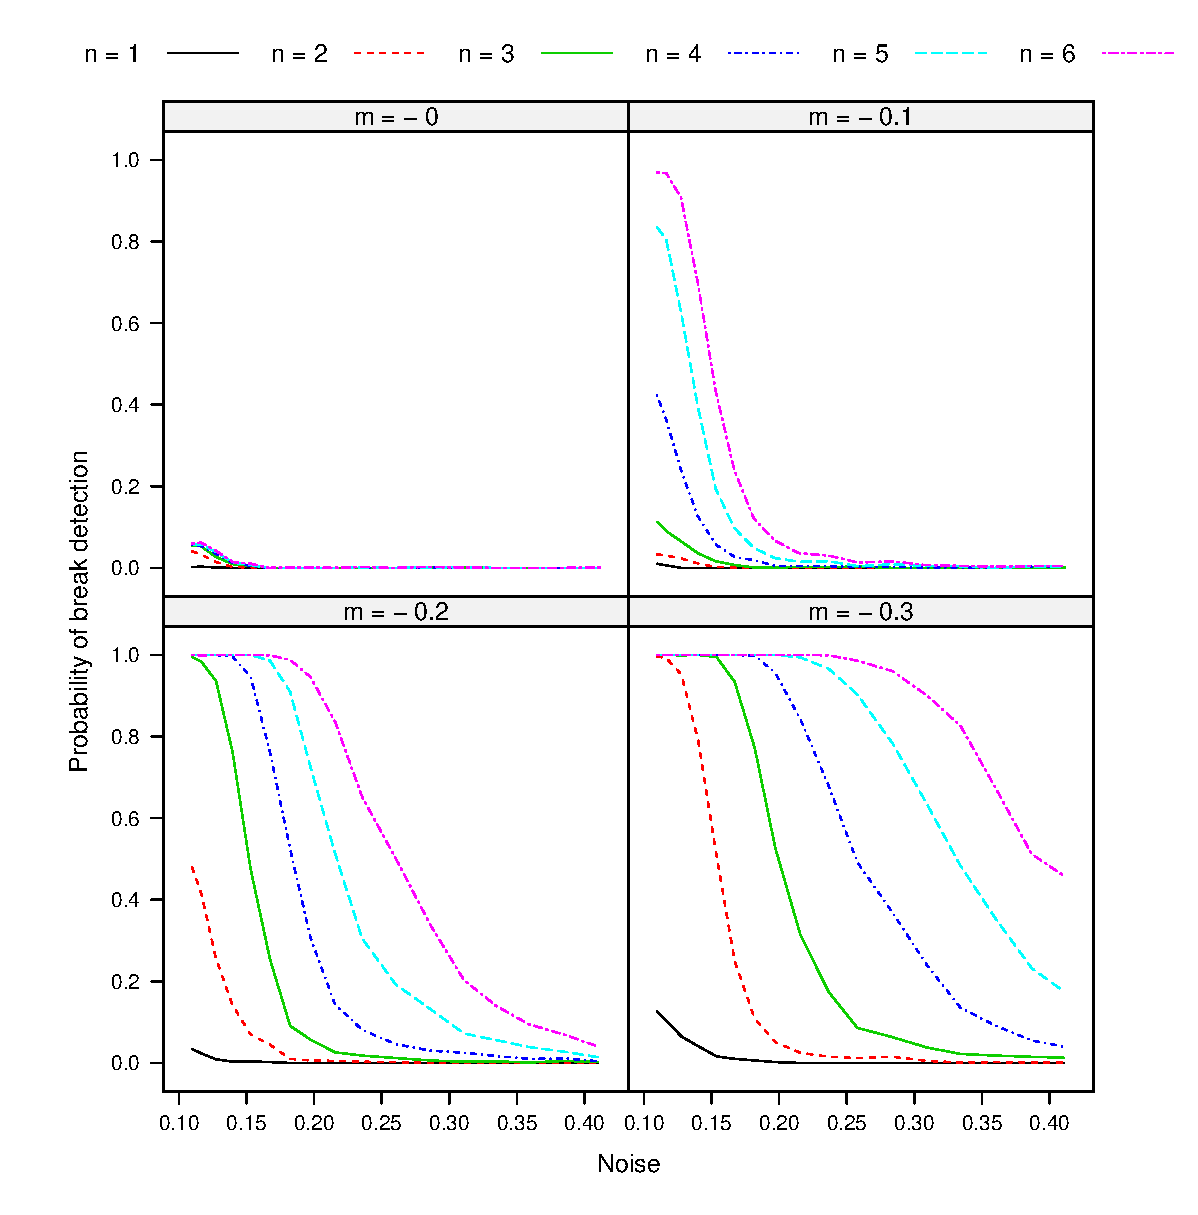
\includegraphics[height=0.9\textwidth]{figs/NrDetections_Time_1000.eps}
  \caption{Results from the simulation experiment (1000 iterations of all different options) illustrating the number of the detected breaks (1000 is the maximum) of the detected breaks using the monitor approach for varying amount of noise, magnitude of change (i.e. dip), and amount of data available in the monitoring period (see description of the simulation experiment for more information about set-up) }
  \label{fig:SimNr}
\end{figure}

\begin{figure}[htp]
\centering
    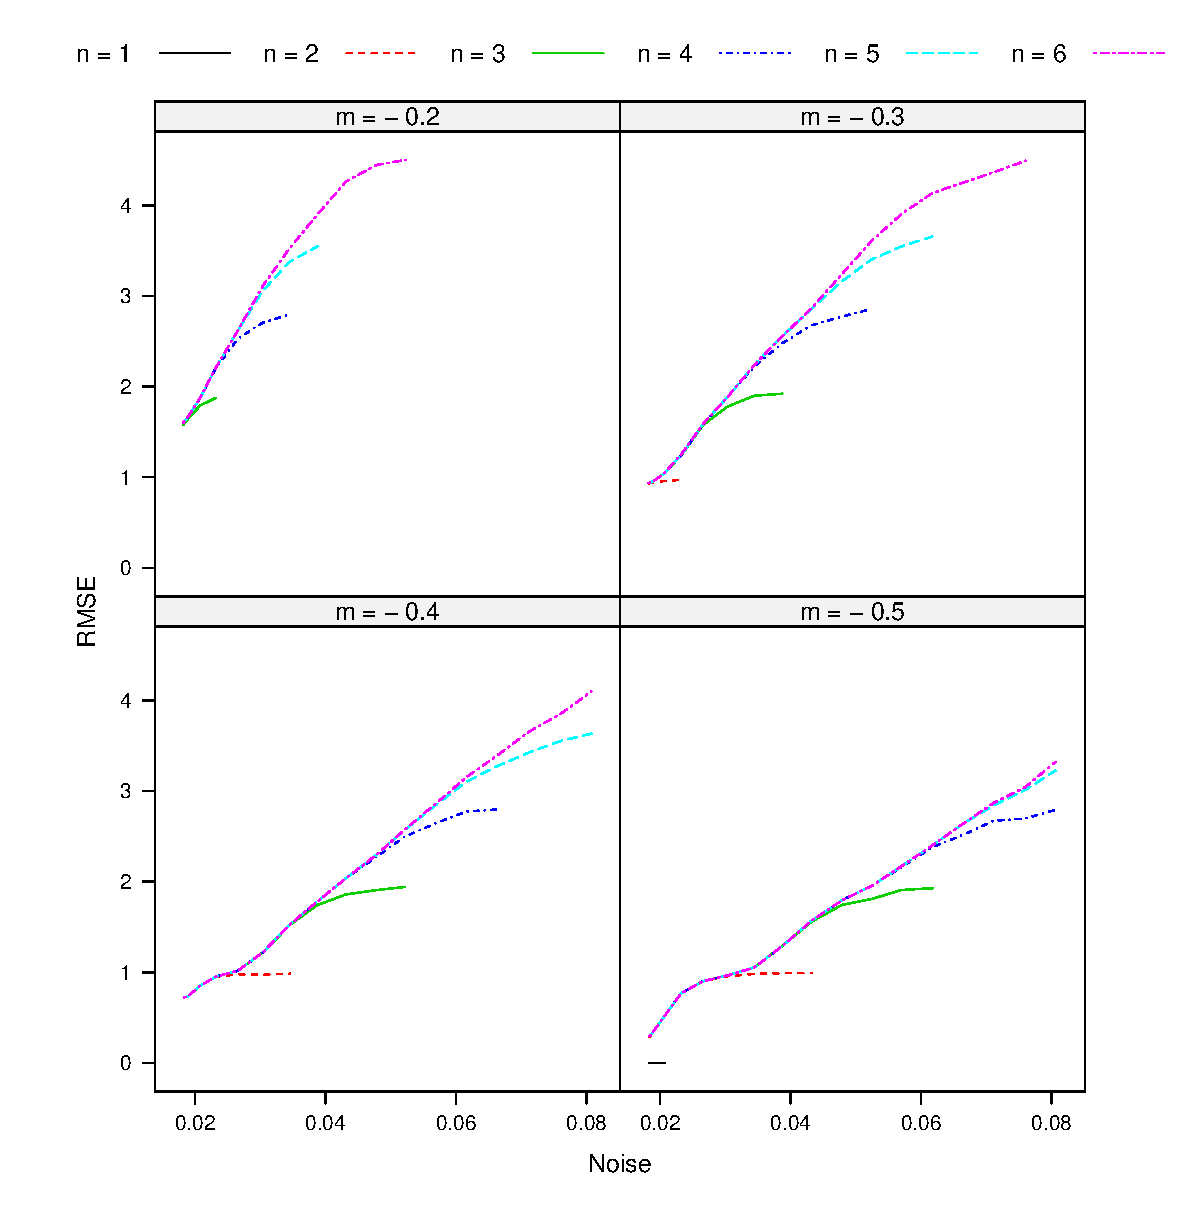
\includegraphics[height=0.9\textwidth]{figs/RMSE_Time_1000.eps}
  \caption{Results from the simulation experiment (1000 iterations of all different options) illustrating the accuracy of time estimation of the detected breaks using the monitor approach for varying amount of noise, magnitude of change (i.e. dip), and amount of data available in the monitoring period (see description of the simulation experiment for more information about set-up) }
  \label{fig:SimRMSE}
\end{figure}

\begin{figure}[htp]
\centering
    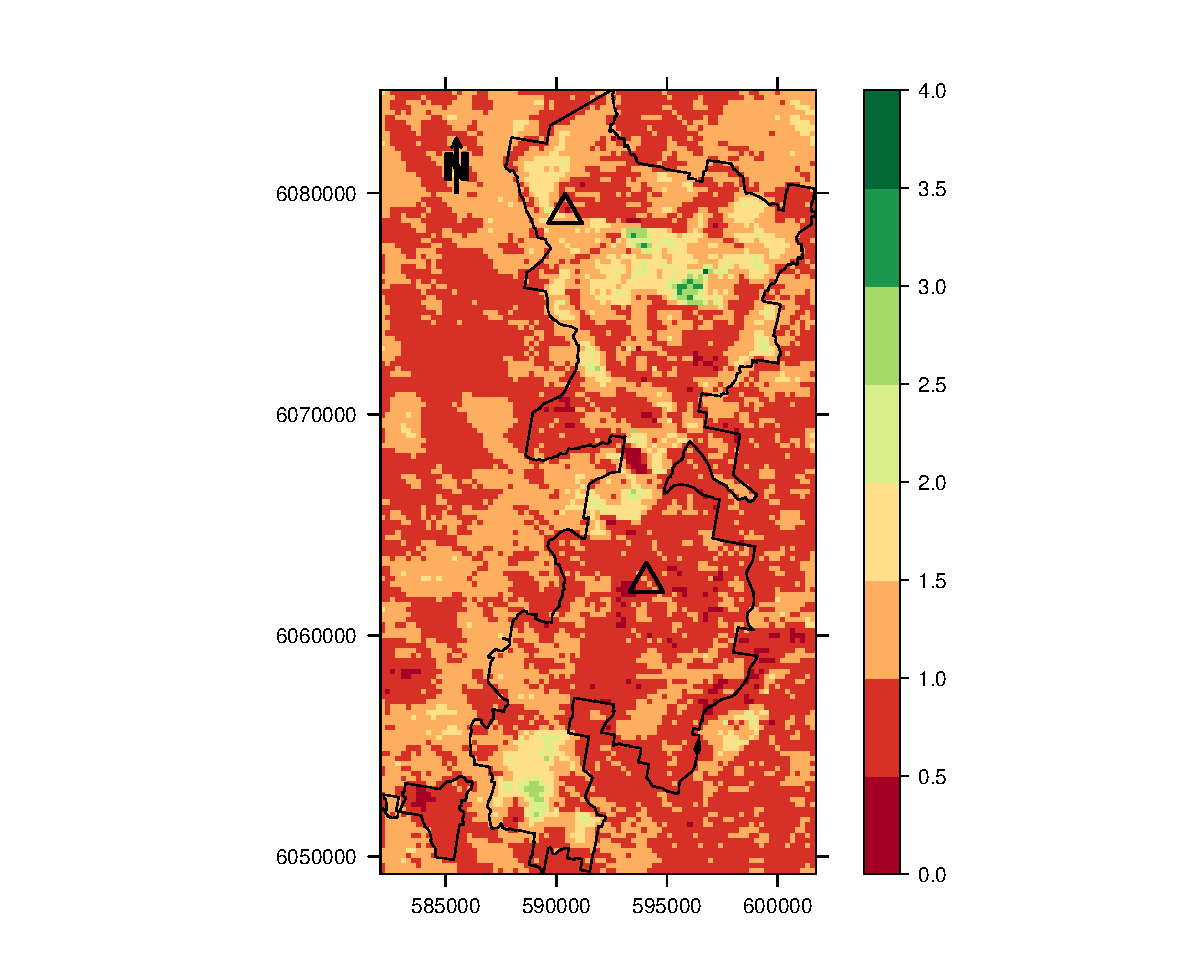
\includegraphics[height=0.9\textwidth]{figs/SignaltoNoiseRatio.eps}
  \caption{Spatial variation of the signal to noise ratio is the study area. (Try out: only for your information - not sure whether I will include this in the paper) }
  \label{fig:SpatSignalNoise}
\end{figure}

\begin{figure}[htp]
\centering
    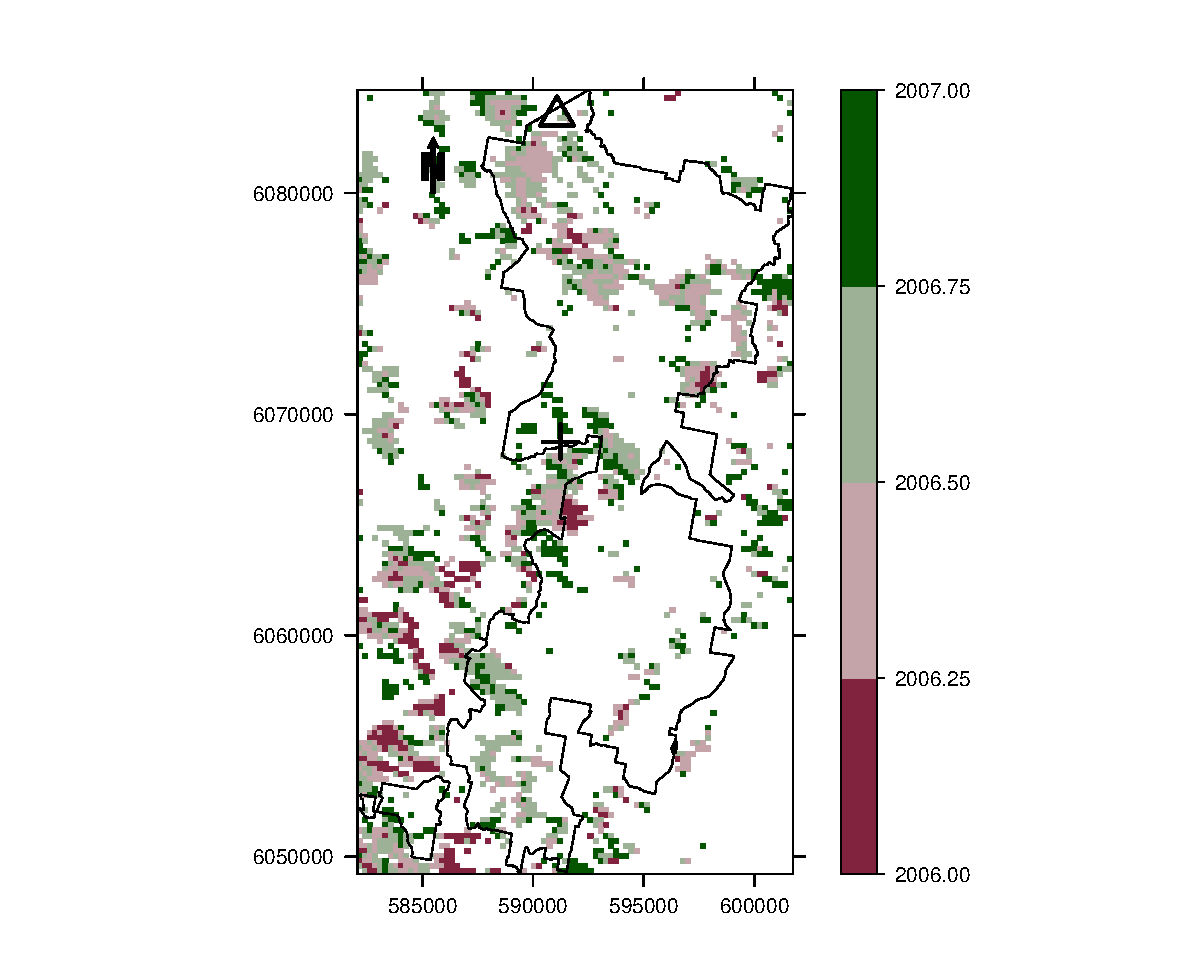
\includegraphics[height=0.9\textwidth]{figs/TimeofChangein2006.eps}
  \caption{ Spatial variation of the Time of change if a break is detected in the study area (no break in 2006 = white) . (only for your information - not sure whether I will include this in the paper) }
  \label{fig:SpatTimeofChange}
\end{figure}

\begin{figure}[htp]
\centering
    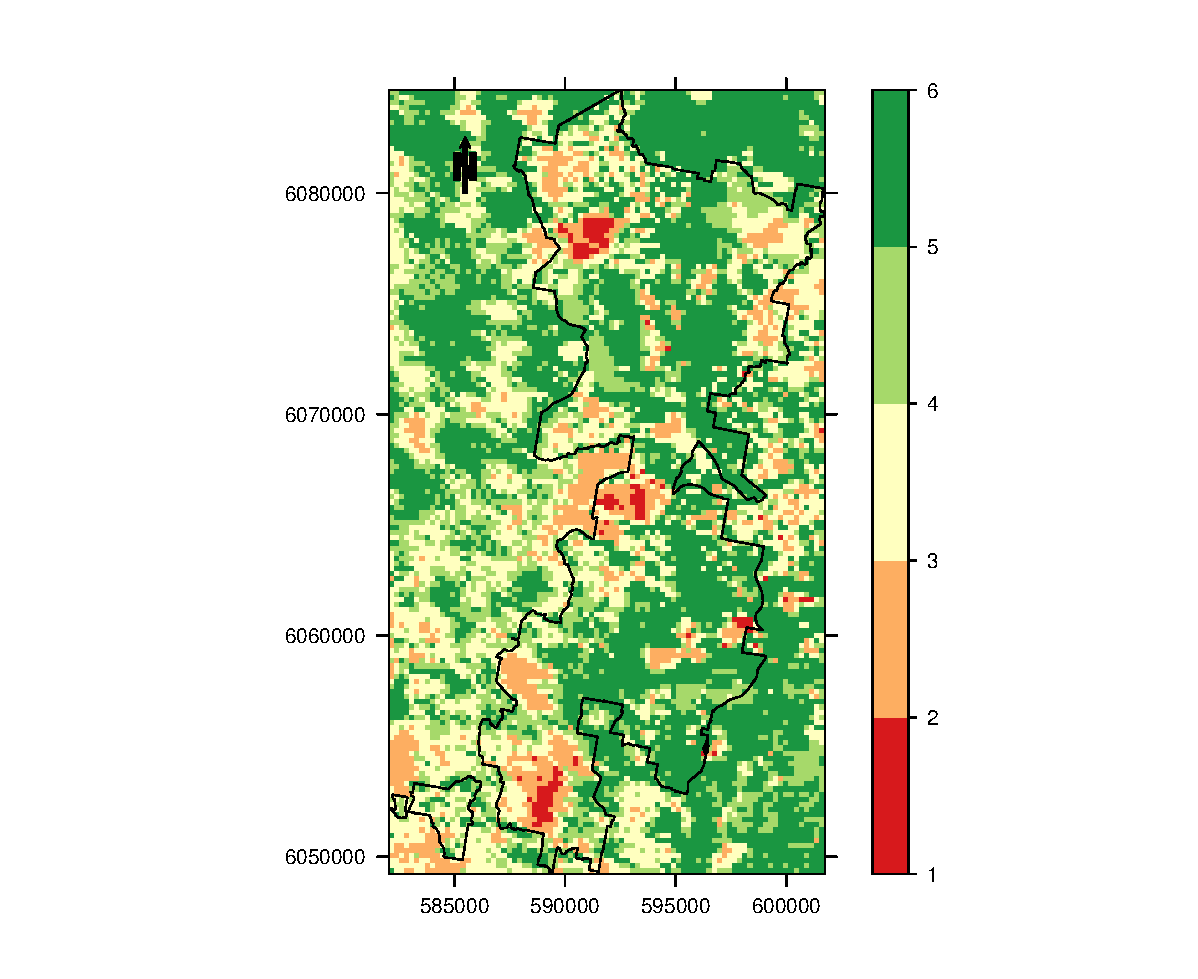
\includegraphics[height=0.9\textwidth]{figs/LengthStableHistory.eps}
  \caption{Spatial variation of the length the stable history period}
  \label{fig:SpatLStableHist}
\end{figure}

\begin{figure}[htp]
\centering
    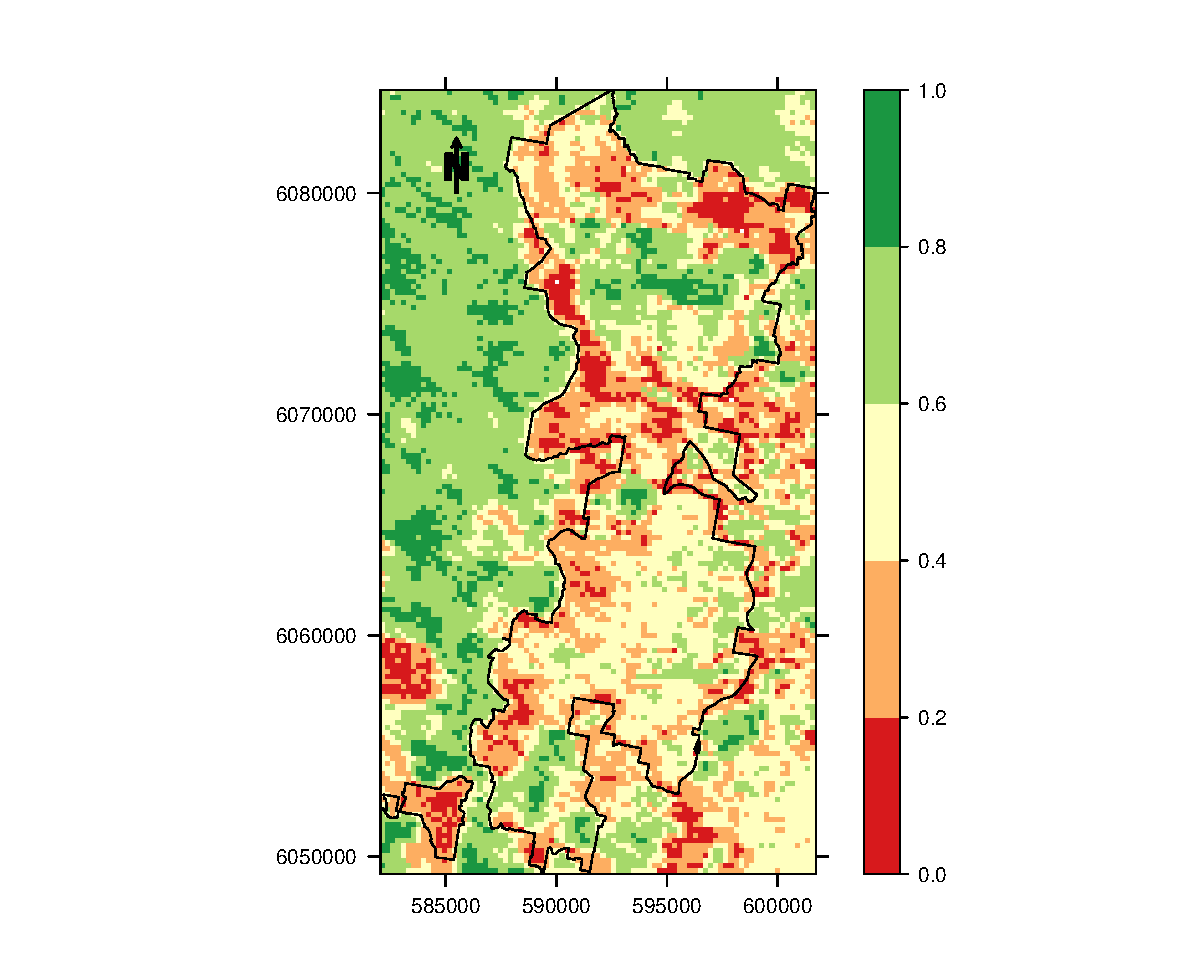
\includegraphics[height=0.9\textwidth]{figs/R2ofthemodelfit.eps}
  \caption{ Spatial variation of the $R^2$ of the model fit which also depend on the length the stable history period}
  \label{fig:SpateR2}
\end{figure}

\end{document}

